\section{Hardware Components}
\subsection{Robotic Arms}

\subsubsection{ABB IRB 120}
The ABB IRB 120 is a compact, high-speed 6-DOF industrial manipulator used for assembly and placement tasks~\cite{abb_irb120}. It provides precise motion control and is mounted to cover the assembly side of the workspace. 
\begin{wrapfigure}{r}{0.44\textwidth} % "r" = right, width = 35% of text
    \vspace{20pt}
    \centering
    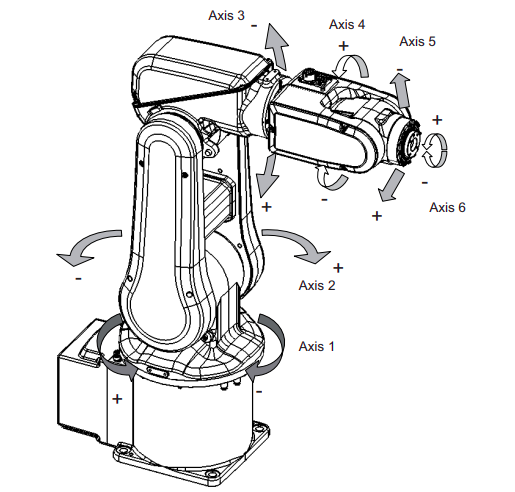
\includegraphics[width=0.44\textwidth]{Figures/chapter3/System_architecture/ABB_axes.png} % put your file here
    \caption{ABB IRB 120 joint axes and DOF layout~\cite{abb_irb120}.}
    \label{fig:abb_axes}
    \vspace{-200pt}
\end{wrapfigure}

\begin{itemize}
    \item \textbf{Model:} ABB IRB 120 (6-DOF articulated arm)
    \item \textbf{Payload Capacity:} 3\,kg
    \item \textbf{Maximum Reach:} 580\,mm
    \item \textbf{Repeatability:} $\pm$0.01\,mm (ISO 9283)
    \item \textbf{Arm Mass:} 25\,kg
    \item \textbf{Motion Speeds:}
        \begin{itemize}
            \item Joint 1–3: up to 250°/s
            \item Joint 4–5: up to 320°/s
            \item Joint 6: up to 420°/s
        \end{itemize}
    \item \textbf{Gripper:} Two-finger parallel gripper
    \item \textbf{Controller:} IRC5 (supports ROS 2 integration via bridge)
    \item \textbf{Mounting:} Floor, inverted, or angled
\end{itemize}

\subsubsection{AR4 MK3}
The AR4 MK3 is a 6-DOF robotic arm developed by Annin Robotics~\cite{ar4_mk3}. It is used for grasping bricks and either directly assembling them or transporting them to the ABB arm for handover. Its open architecture allows integration of custom sensors and control modules.
\\\begin{wrapfigure}{r}{0.35\textwidth} % "r" = right, width = 35% of text
    \vspace{20pt}
    \centering
    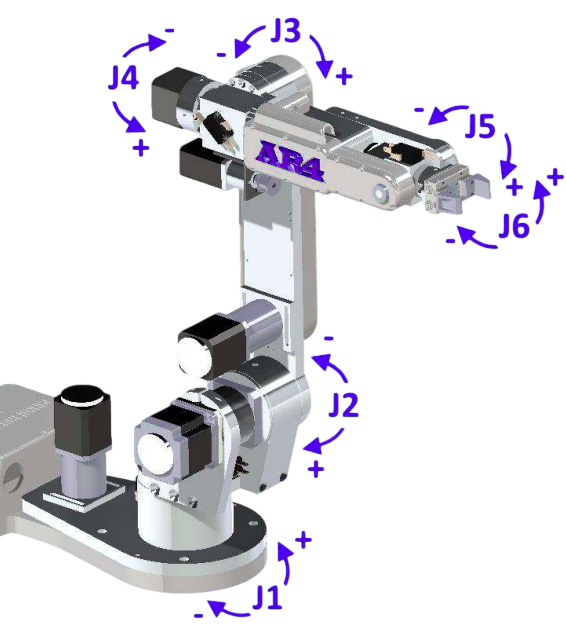
\includegraphics[width=0.35\textwidth]{Figures/chapter3/System_architecture/AR4_axes.png} % put your file here
    \caption{AR4 MK3 joint axes and DOF layout~\cite{ar4_mk3}.}
    \label{fig:ar4_axes}
    \vspace{-200pt}
\end{wrapfigure}
\begin{itemize}
    \item \textbf{Model:} AR4 MK3 (6-DOF articulated arm)
    \item \textbf{Payload Capacity:} 1–2\,kg
    \item \textbf{Repeatability:} $\approx$0.2\,mm
    \item \textbf{Structure:} Aluminum/3D-printed links with stepper motors
    \item \textbf{End-Effector:} Two-finger gripper (ESP32 controlled)
    \item \textbf{Eye-in-Hand Camera:} ESP32-CAM mounted for local perception
    \item \textbf{Controller:} Arduino/Teensy microcontroller
    \item \textbf{Communication:} ROS 2 action servers for point control and visual servo
\end{itemize}

\subsection{Encoders and Joint Feedback}

\subsubsection{ABB IRB 120 Encoders:}
\begin{itemize}
    \item \textbf{Type:} Absolute, multi-turn encoders integrated in each joint.
    \item \textbf{Resolution:} 0.001° (for joint motion, from IRC5 datasheet~\cite{abb_irb120}).
    \item \textbf{Purpose:} Provides precise joint position feedback for high-accuracy motion control, repeatability, and trajectory execution.
    \item \textbf{Integration:} Fully interfaced with IRC5 controller; supports ROS~2 via ABB-ROS2 bridge for motion planning and calibration.
\end{itemize}

\subsubsection{AR4 MK3 Encoders:}
\begin{itemize}
    \item \textbf{Type:} Magnetic absolute encoders at each joint.
    \item \textbf{Resolution:} 12-bit per joint (approx. 0.088° resolution).
    \item \textbf{Purpose:} Joint position feedback for closed-loop control, calibration, and fine-grained motion during visual servoing.
    \item \textbf{Integration:} Connected to AR4’s control board and ROS~2 nodes for motion and IBVS control.
\end{itemize}

\subsection{Cameras and Perception}

\subsubsection{Intel RealSense D435i (Global Perception)}
The RealSense D435i provides global workspace perception, including depth and RGB streams for segmentation and pose estimation~\cite{realsense_d435i}.
\\\begin{wrapfigure}{r}{0.33\textwidth} % "r" = right, width = 35% of text
    \vspace{-40pt}
    \centering
    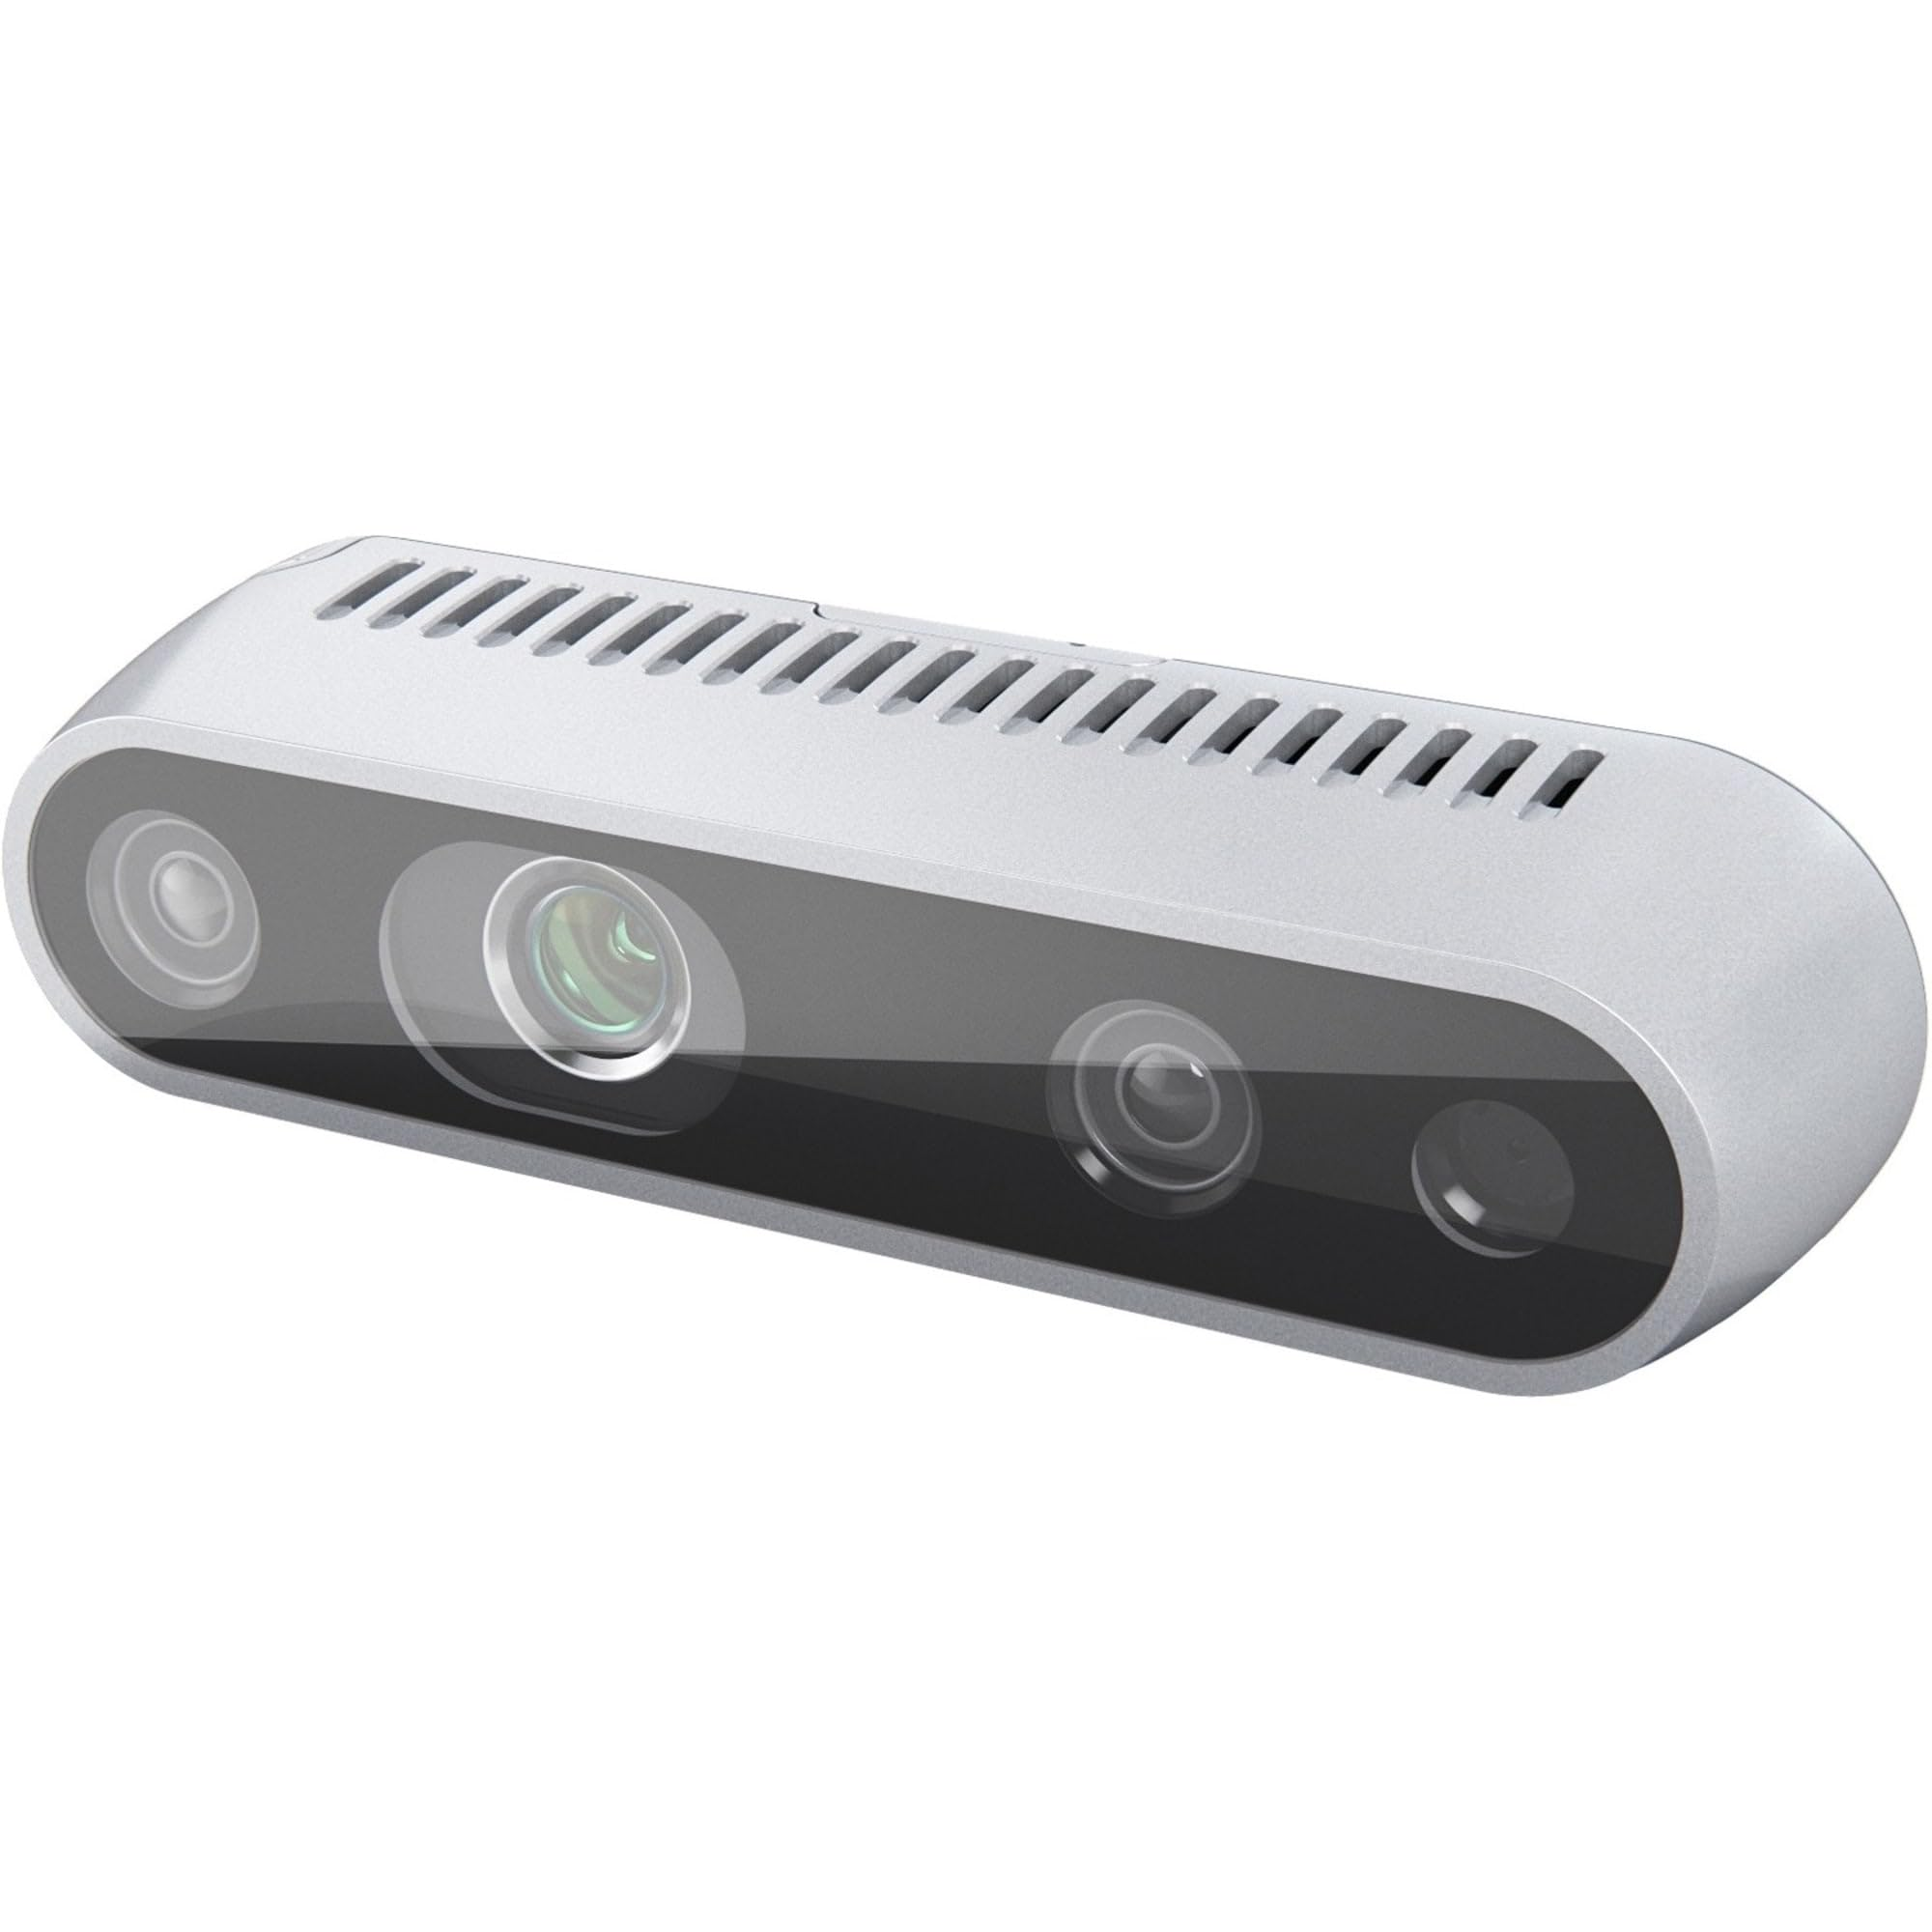
\includegraphics[width=0.33\textwidth]{Figures/chapter3/System_architecture/Realsense.jpg} % put your file here
    \caption{RealSense D435i~\cite{realsense_d435i}.}
    \label{fig:realsense}
    \vspace{-200pt}
\end{wrapfigure}
\begin{itemize}
    \item \textbf{Placement:} Fixed above assembly table
    \item \textbf{Output:} RGB + depth images for YOLOv8 segmentation
    \item \textbf{Frame Rate:} 30\,Hz
    \item \textbf{Calibration:} Camera-to-ABB-base transformation in TF2
\end{itemize}

\subsubsection{ESP32-CAM Eye-in-Hand Camera}

An ESP32-CAM module equipped with an OV2640 image sensor is mounted on the AR4 Mk3 end-effector to provide local visual feedback during the final approach and grasping phase. This eye-in-hand configuration enables fine alignment through image-based visual servoing (IBVS), complementing the global perception provided by the overhead camera.
\\\begin{wrapfigure}{r}{0.33\textwidth} % "r" = right, width = 35% of text
    \vspace{0pt}
    \centering
    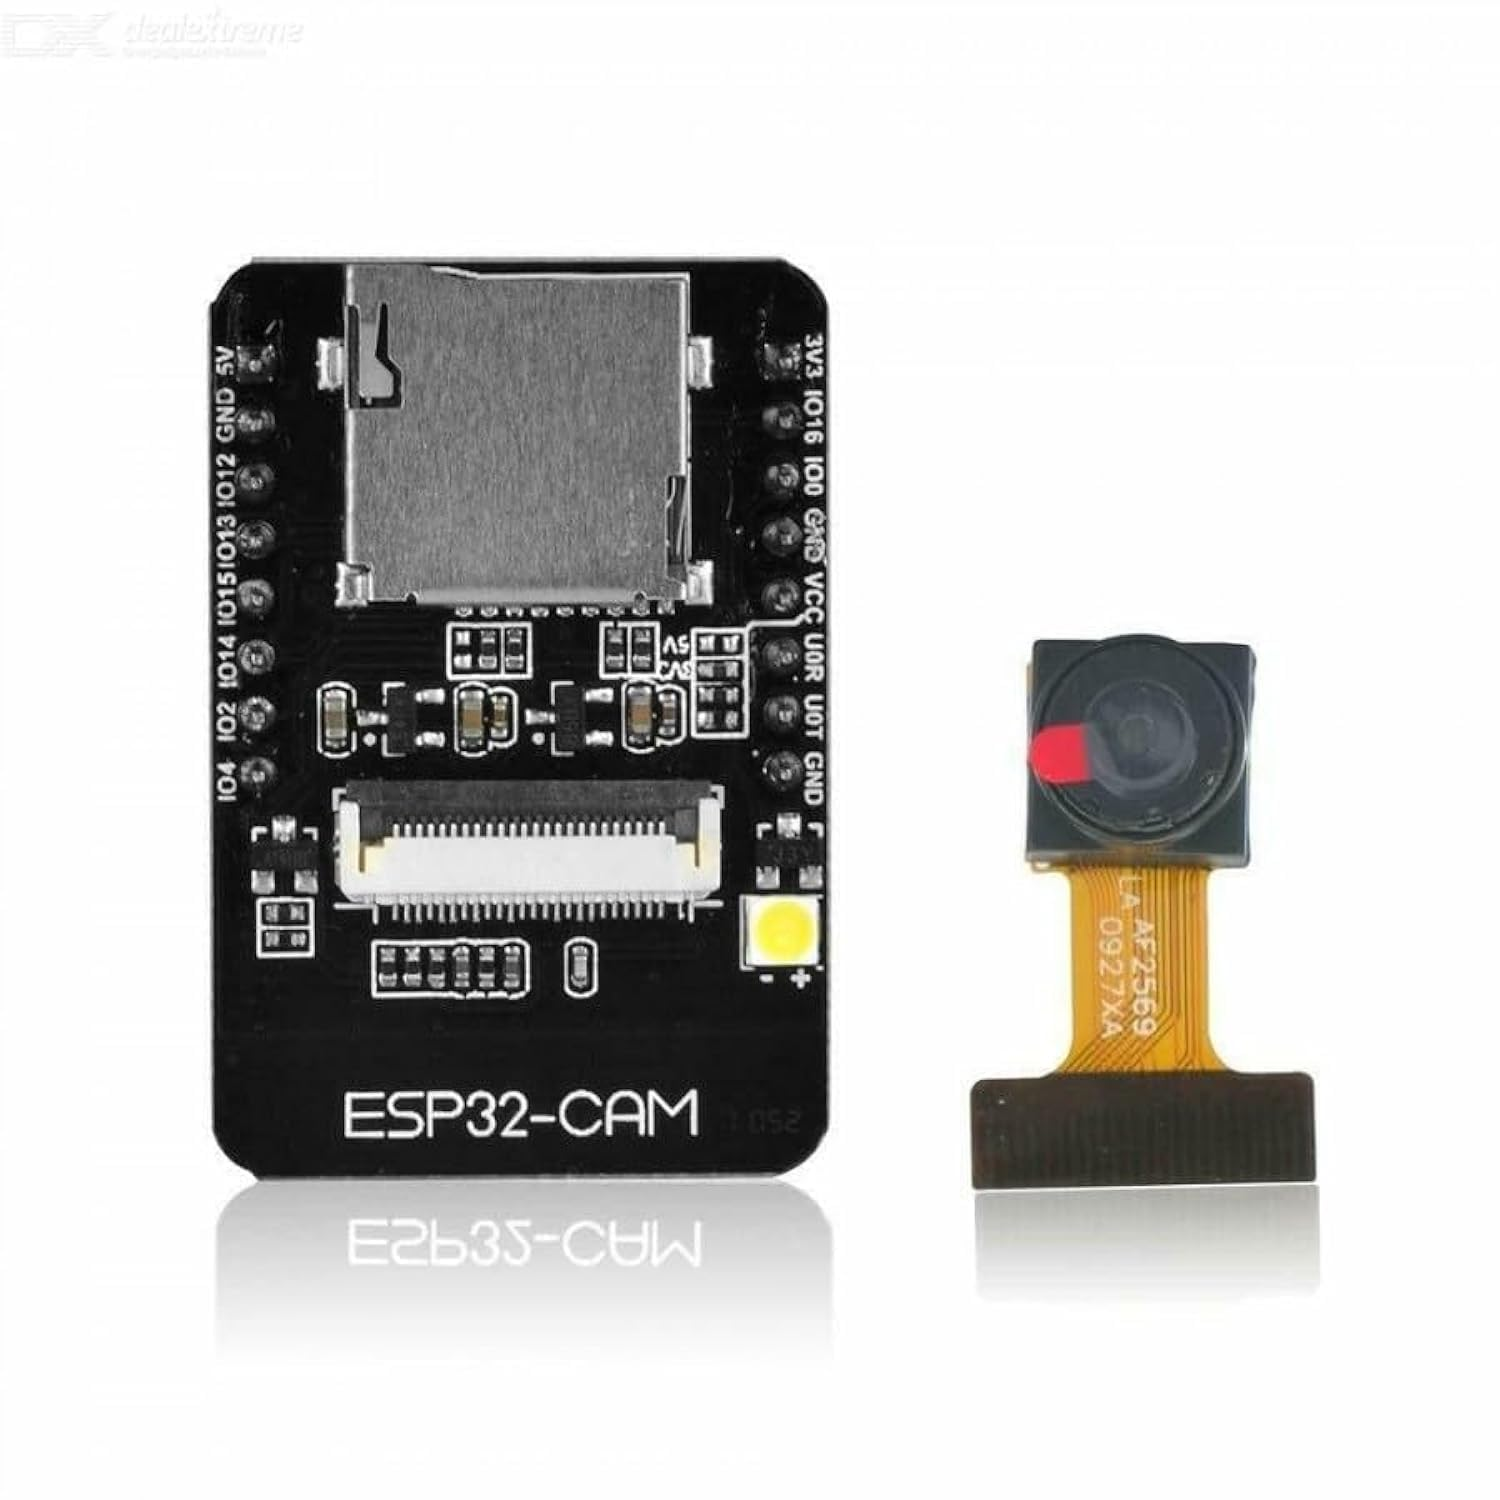
\includegraphics[width=0.33\textwidth]{Figures/chapter3/System_architecture/ESP-CAM.jpg} % put your file here
    \caption{ESP32-CAM OV2640~\cite{OV2640Datasheet}.}
    \label{fig:espcam}
    \vspace{-80pt}
\end{wrapfigure}

\begin{itemize}
    \item \textbf{Sensor:} OV2640 CMOS image sensor.
    \item \textbf{Resolution:} 640 $\times$ 480 pixels (VGA).
    \item \textbf{Lens:} Wide-angle fisheye lens with approximately $160^{\circ}$ field of view.
    \item \textbf{Mounting:} Rigidly attached to the AR4 end-effector, aligned with the gripper frame.
    \item \textbf{Frame Rate:} 20--25 Hz, limited by onboard processing and wireless transmission.
\end{itemize}

Due to the wide-angle fisheye lens, the camera exhibits significant radial distortion. Therefore, a fisheye camera model was adopted during calibration. The intrinsic parameters were obtained offline and include the camera matrix and distortion coefficients, enabling accurate image rectification and metric interpretation of image features. The calibrated intrinsic parameters are used within the visual servoing pipeline to reduce systematic projection errors during closed-loop control.

The camera is primarily used for local feature tracking and alignment rather than global pose estimation. Its relatively low resolution and latency (approximately 100--200 ms) are mitigated through low-gain feedback control and the limited motion range during the final grasping phase. Despite these limitations, the eye-in-hand camera provides sufficient accuracy for correcting residual positioning errors introduced by kinematic uncertainties in the AR4 robot.

The OV2640 camera module and lens specifications are consistent with commercially available ESP32-CAM systems commonly used in embedded vision applications \cite{OV2640Datasheet}.

